% 1987 年广东卷理工农医类第二卷第二题：三棱台
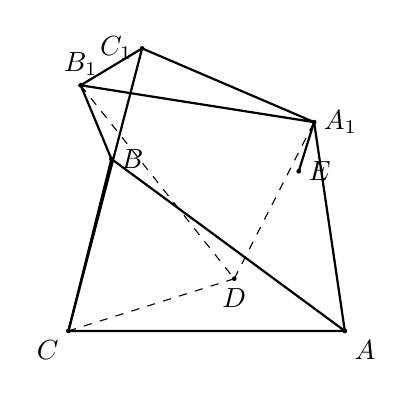
\begin{tikzpicture}[scale=0.78,>=stealth]
  \coordinate (A) at (4.5,0);
  \coordinate (C) at (0,0);
  \coordinate (B) at (0.7,2.8);
  \coordinate (A1) at (4.0,3.4);
  \coordinate (C1) at (1.2,4.6);
  \coordinate (B1) at (0.2,4.0);
  \coordinate (D) at (2.7,0.85);
  \coordinate (E) at (3.75,2.6);
  \draw[thick] (A)--(B)--(C)--(A);
  \draw[thick] (A1)--(B1)--(C1)--(A1);
  \draw[thick] (A)--(A1) (B)--(B1) (C)--(C1);
  \draw[dashed] (B1)--(D) (D)--(A1) (D)--(C);
  \draw[thick] (E)--(A1);
  \fill (A) circle (1.1pt) node[below right] {$A$};
  \fill (B) circle (1.1pt) node[right] {$B$};
  \fill (C) circle (1.1pt) node[below left] {$C$};
  \fill (A1) circle (1.1pt) node[right] {$A_1$};
  \fill (B1) circle (1.1pt) node[above] {$B_1$};
  \fill (C1) circle (1.1pt) node[left] {$C_1$};
  \fill (D) circle (1.1pt) node[below] {$D$};
  \fill (E) circle (1.1pt) node[right] {$E$};
\end{tikzpicture}
